\chapter{Generazione dei Segnali Principali}

%--------------------------------------------------------------------------------------------

Per la generazione dei segnali a rampa e a triangolo si decide di procedere in ogni caso
per via digitale, utilizzando dei contatori binari abbinati ad un convertitore
digitale-analogico.
\medskip

\begin{figure}[ht]
    \centering
    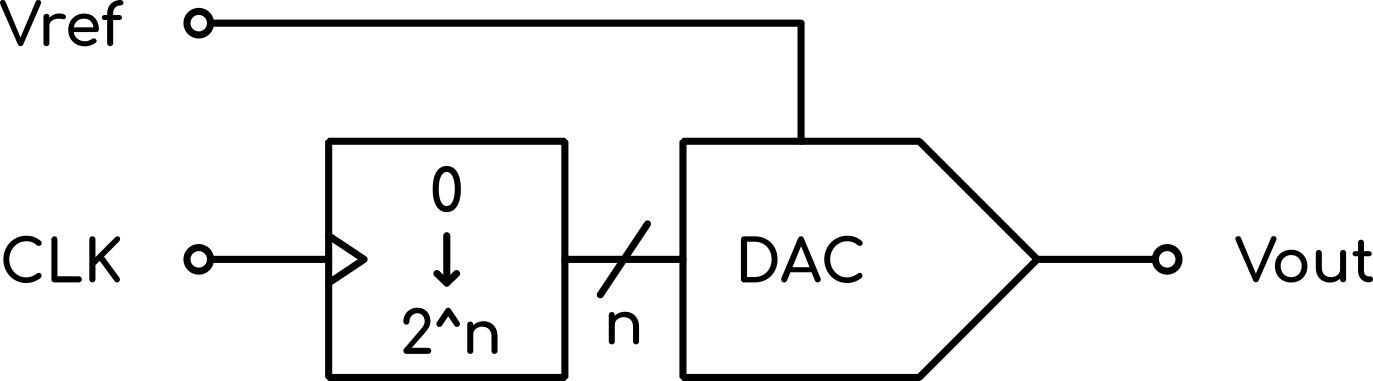
\includegraphics{block_diagrams/counter_block_diagram.png}
    \caption{Schema a blocchi generale di un generatore di segnale}
    \label{counter_block_diagram}
\end{figure}

%--------------------------------------------------------------------------------------------

\section{Rampa}

%--------------------------------------------------------------------------------------------

\subsection*{Principio di Funzionamento}

%--------------------------------------------------------------------------------------------

Per il segnale a rampa si fa uso di un contatore unidirezionale, ovvero un dispositivo
in grado di contare automaticamente da $0$ a $2^n$, dove $n$ corrisponde al numero di bit,
semplicemente fornendo un segnale di clock adeguatamente dimensionato. Maggiore il numero
di bit $n$, maggiore sarà la precisione del nostro segnale, quindi minore l'intensità del
rumore generato.
\medskip

\begin{figure}[ht]
    \centering

    \begin{subfigure}{.5\textwidth}
        \centering
        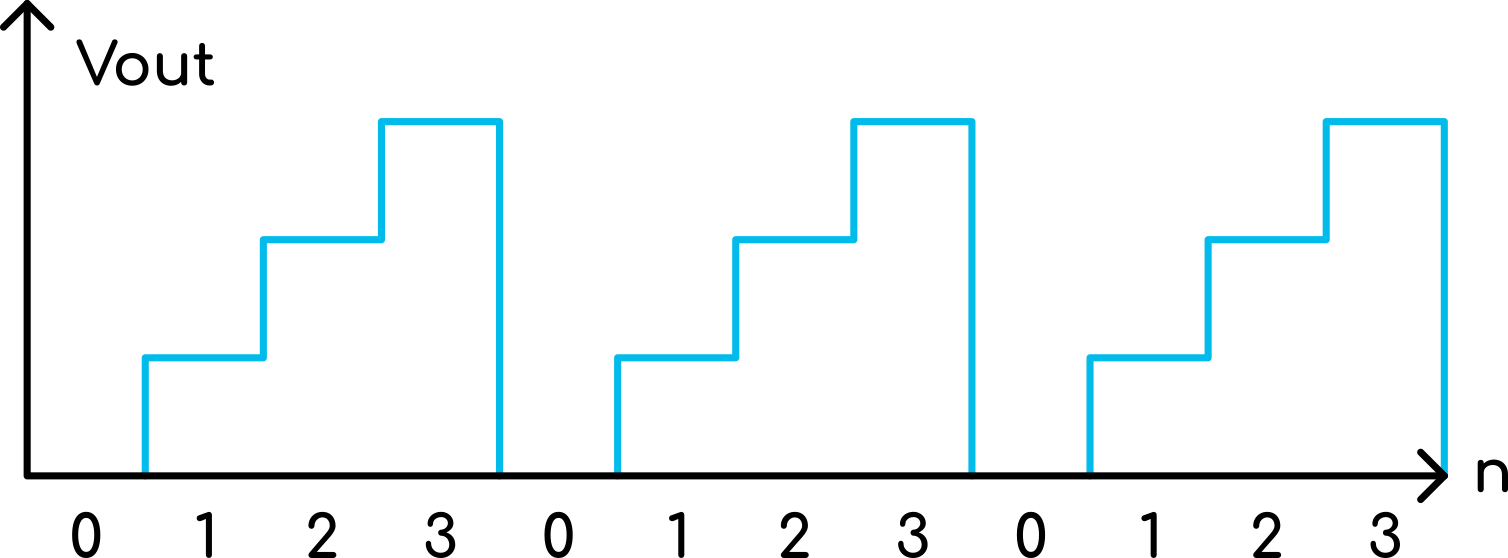
\includegraphics{graphs/low_res_ramp.png}
        \caption{Rampa ottenuta con un contatore a 2 bit}
        \label{low_res_ramp}
    \end{subfigure}%
    \begin{subfigure}{.5\textwidth}
        \centering
        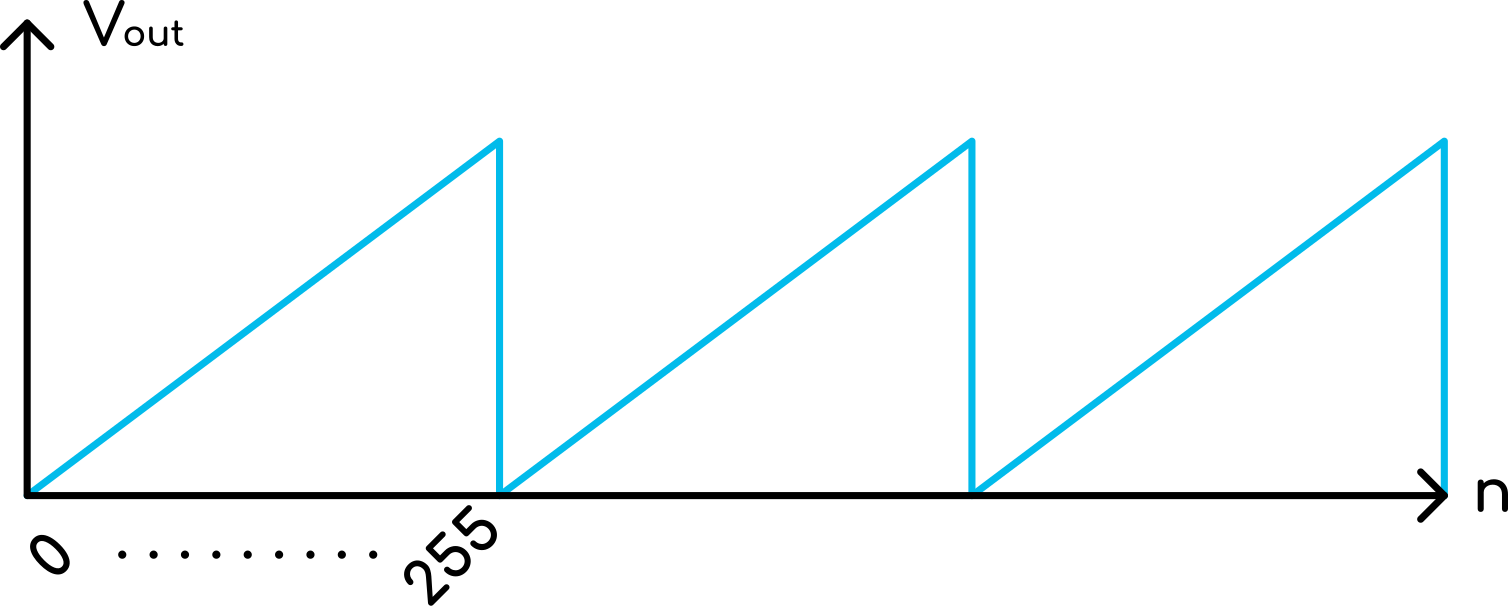
\includegraphics{graphs/high_res_ramp.png}
        \caption{Rampa ottenuta con un contatore a 8 bit}
        \label{high_res_ramp}
    \end{subfigure}

    \caption{Confronto tra contatori unidirezionali con diverso numero di bit}
    \label{ramps}
\end{figure}

Tuttavia aumentando il numero di bit del contatore è facile intuire che, a parità di
frequenza del segnale in uscita, la frequenza del segnale di clock debba necessariamente
aumentare.

Vale infatti la seguente relazione:

\begin{displaymath}
    f_{signal}=\frac{f_{clk}}{2^n}[Hz]
\end{displaymath}

poichè il contatore deve effettuare un conteggio completo durante un periodo del segnale
in uscita. Questo implica dunque un limite massimo al numero di bit del contatore.

La quantità di bit utilizzati per l'applicazione è $8$, valore che ci consente di limitare
al $MHz$ la frequenza di clock, contare fino a $255$ e dividere l'intervallo di tensione
d'uscita in altrettanti livelli, ottenendo quindi una variazione di

\begin{displaymath}
    V_{step}=\frac{2V_{ref}}{2^n}=\frac{10V}{256}\approx39mV
\end{displaymath}


per ogni singolo bit (scegliendo $V_{ref}=+5V$).
\medskip

\begin{figure}[ht]
    \centering
    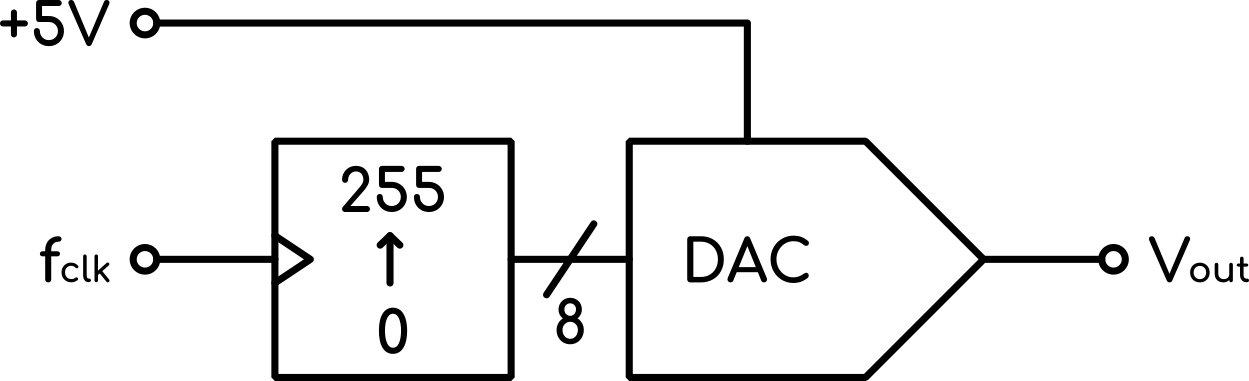
\includegraphics{block_diagrams/ramp_block_diagram.png}
    \caption{Schema a blocchi del sottosistema per la generazione della rampa}
    \label{ramp_block_diagram}
\end{figure}

A questo punto possiamo calcolare le speccifiche del segnale di clock da generare,
andando a vedere quali sono le frequenze desiderate per i segnali audio:

\begin{itemize}
    \item Valore minimo (nota A0): $f_{signal-min}=27.5Hz\rightarrow f_{clk-min}\approx7kHz$
          a cui corrisponderà un ingresso di $0V$;
    \item Valore massimo (nota A8): $f_{signal-max}\approx7kHz\rightarrow f_{clk-max}\approx1.8MHz$
          a cui corrisponderà un ingresso di $8V$;
\end{itemize}

ovvero un range di funzionamento esteso lungo 8 ottave.

%--------------------------------------------------------------------------------------------

\subsection*{Componenti Utilizzati e Schemi Elettrici}

%--------------------------------------------------------------------------------------------

Si passa ora alla scelta dei componenti per la realizzazione del blocco circuitale.

\begin{itemize}
    \item Contatore: 74HC590 \cite{74hc590};
    \item DAC: DAC0800 \cite{dac0800};
\end{itemize}

Per il circuito DAC si utilizza lo schema a pg.10 del relativo datasheet del componente.
Tale configurazione ci permette infatti di convertire il dato binario in un valore compreso
nell'intervallo $\pm V_{ref}= \pm 5V$, tuttavia si utilizzano un amplificatore
operazionale e dei resistori di valore differente (rispettivamente TL074 \cite{tl074} e
$R_L=\bar{R_L}=3.3k\Omega$). Si noti che anche $V_{ref}$ viene scelta diversa rispetto allo
schema nel datasheet ($+5V$), in modo da garantire le specifiche di progetto sul segnale
in uscita.
\medskip

\begin{figure}[ht]
    \centering
    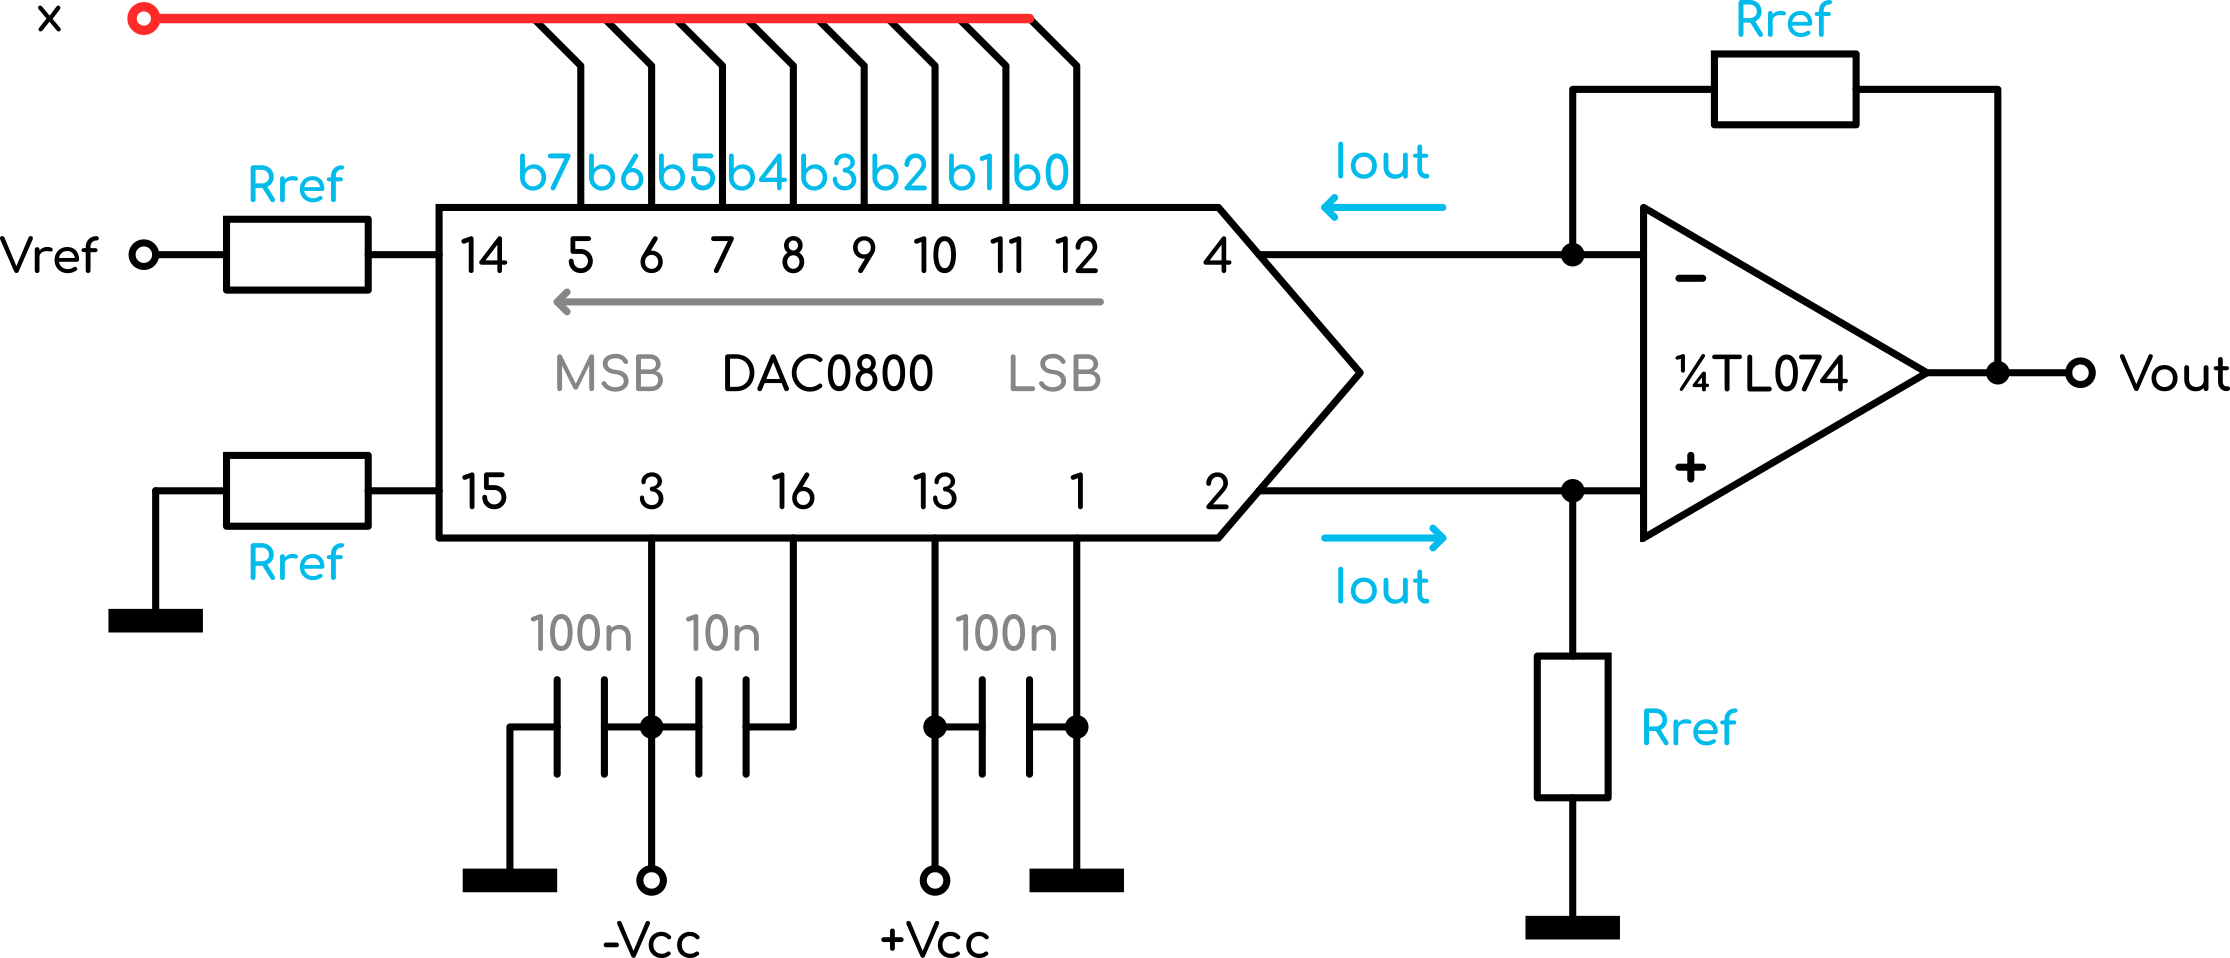
\includegraphics{circuits/DAC_circuit.png}
    \caption{Schema elettrico del DAC, $\pm V_{cc}=\pm 12V$}
    \label{DAC_circuit}
\end{figure}

Il DAC eroga una corrente $I_{out}$ proporzionale all'ingresso digitale $x$, che viene poi
convertita in una tensione con un operazionale. Le due grandezze sono legate dalla seguente
relazione:

\begin{displaymath}
    V_{out}=V_{ref}\left(\frac{2x-255}{256}\right)=5\left(\frac{2x-255}{256}\right)[V]
\end{displaymath}

Il contatore invece viene collegato nel seguente modo:
\medskip

\begin{figure}[ht]
    \centering
    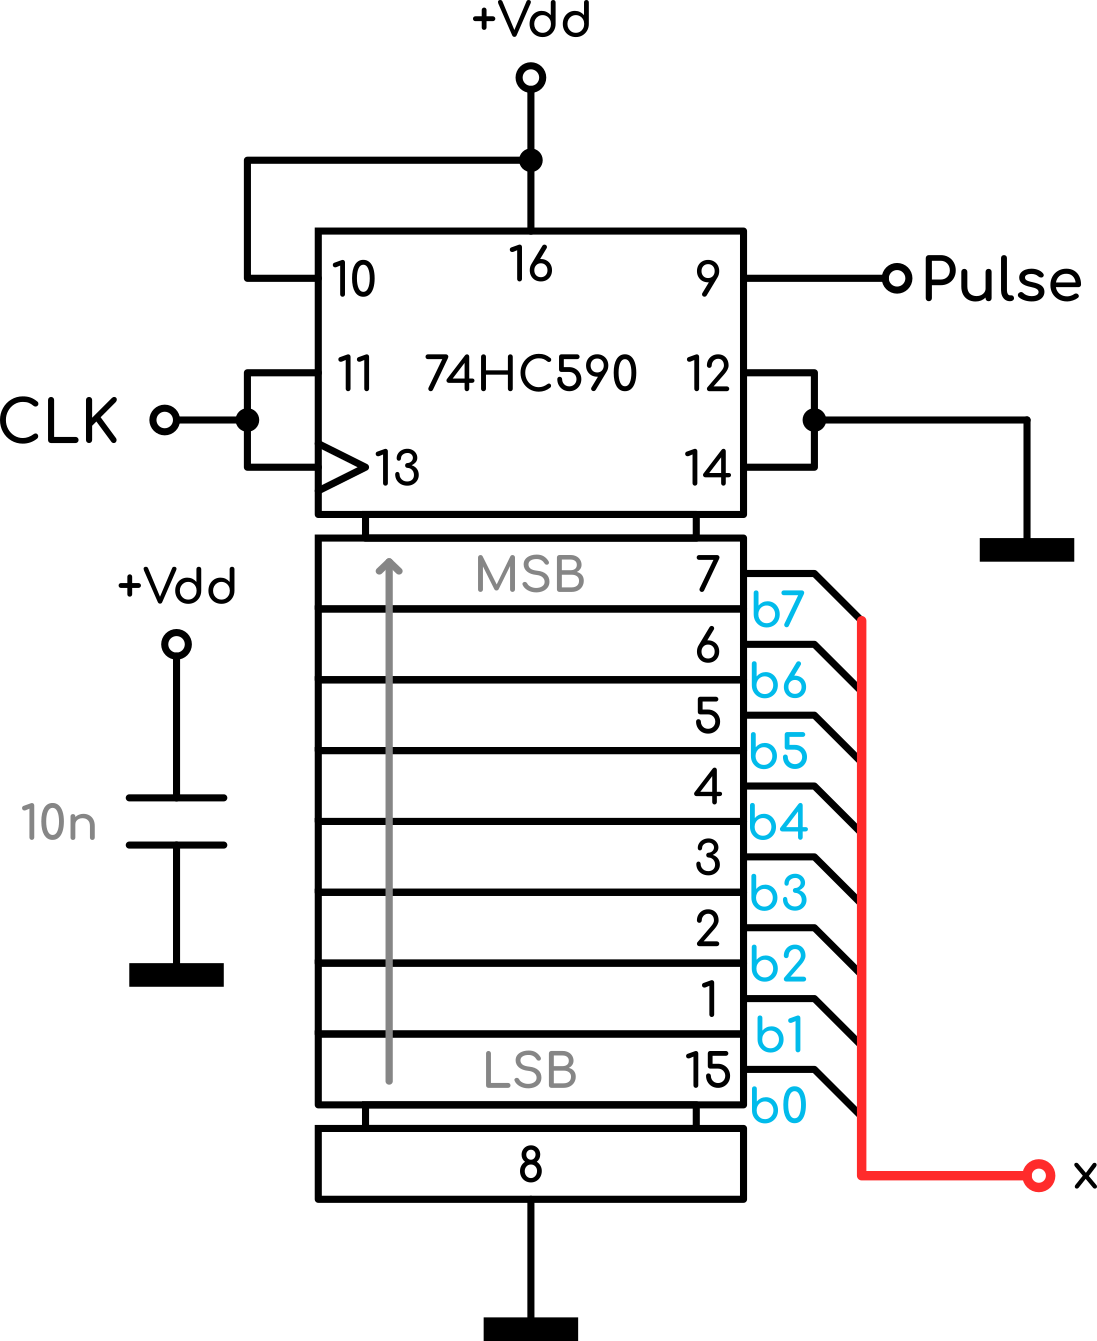
\includegraphics{circuits/ramp_counter_circuit.png}
    \caption{Schema elettrico del contatore per l'onda a rampa, $V_{dd}=+5V$}
    \label{ramp_counter_circuit}
\end{figure}

Si noti l'uscita "Pulse" in figura \ref{ramp_counter_circuit} dalla quale viene prelevato
il segnale a impulso precedentemente accennato, discusso più in dettaglio nel capitolo.
%\ref{ch_impulso}.

Collegando i due blocchi insieme quindi, l'andamento di $V_{out}$ sarà simile a quello
rappresentato in figura \ref{high_res_ramp} e ad ogni impulso di clock corrisponderà un
gradino di tensione di circa $40mV$ come calcolato precendentemente.

%--------------------------------------------------------------------------------------------

\subsection*{Risultati Pratici}

%--------------------------------------------------------------------------------------------

Andiamo ora a verificare la correttezza del circuito realizzato. Il setup di misura è il
seguente:
\medskip

% immagine setup misure rampa

Si osservano le seguenti forme d'onda:
\medskip

\begin{figure}[ht]
    \centering

    \begin{subfigure}{.5\textwidth}
        \centering
        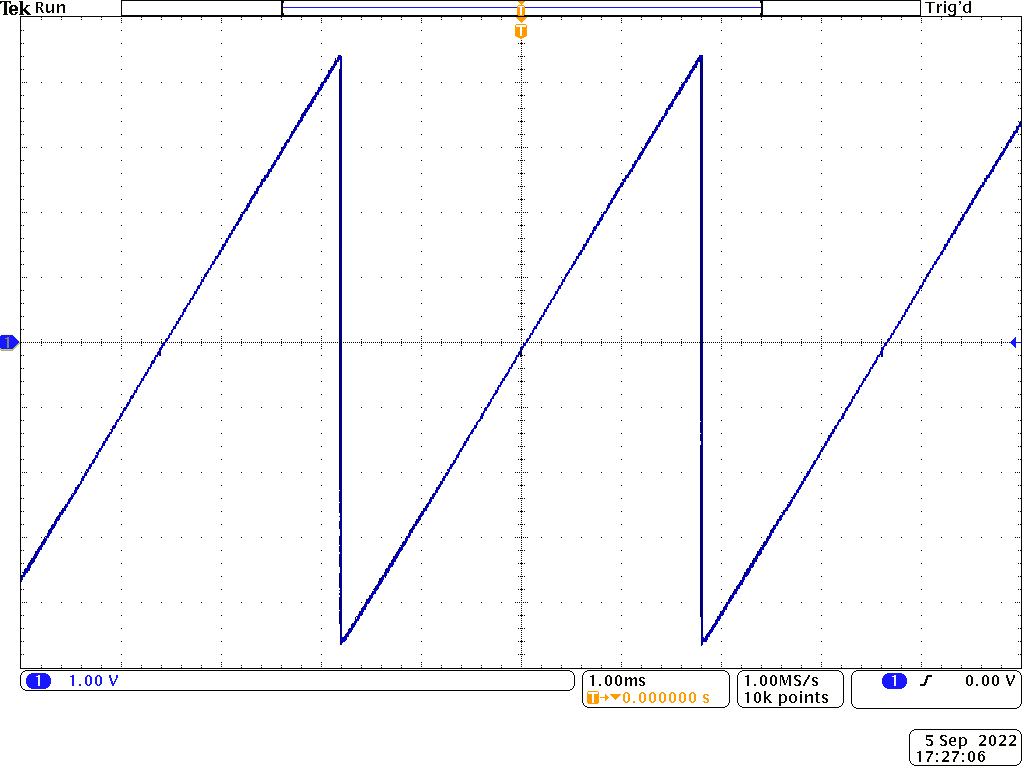
\includegraphics[scale = 0.2]{acquisitions/ramp_wave.png}
        \caption{Acquisizione del segnale a rampa reale}
        \label{acq_ramp}
    \end{subfigure}%
    \begin{subfigure}{.5\textwidth}
        \centering
        
\includegraphics{misc/oscilloscope_placeholder.png}
        \caption{Zoom degli step della rampa acquisita e clock}
        \label{acq_ramp_steps}
    \end{subfigure}

    \caption{Acquisizioni del segnale a rampa}
    \label{acq_ramp_signals}
\end{figure}

%--------------------------------------------------------------------------------------------

\section{Triangolo}

%--------------------------------------------------------------------------------------------

\subsection*{Principio di Funzionamento}

%--------------------------------------------------------------------------------------------

Il ragionamento è del tutto analogo a quello del contatore per la rampa, tuttavia in questo
caso il contatore utilizzato è bidirezionale e necessita di un segnale che determini la
direzione di conteggio (up o down).
\medskip

\begin{figure}[ht]
    \centering
    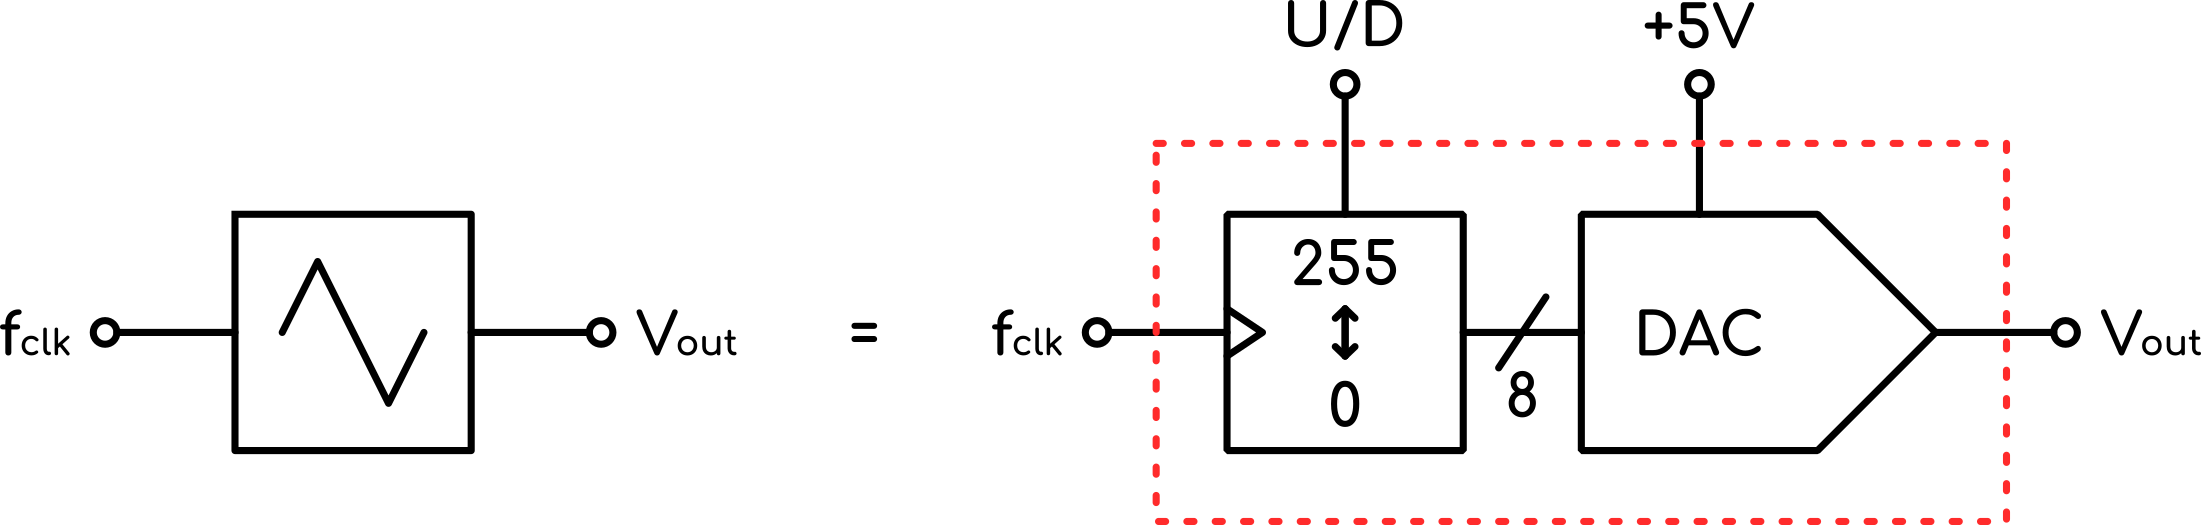
\includegraphics{block_diagrams/triangle_block_diagram.png}
    \caption{Schema a blocchi del sottosistema per la generazione del triangolo}
    \label{triangle_block_diagram}
\end{figure}

\begin{figure}[ht]
    \centering

    \begin{subfigure}{.5\textwidth}
        \centering
        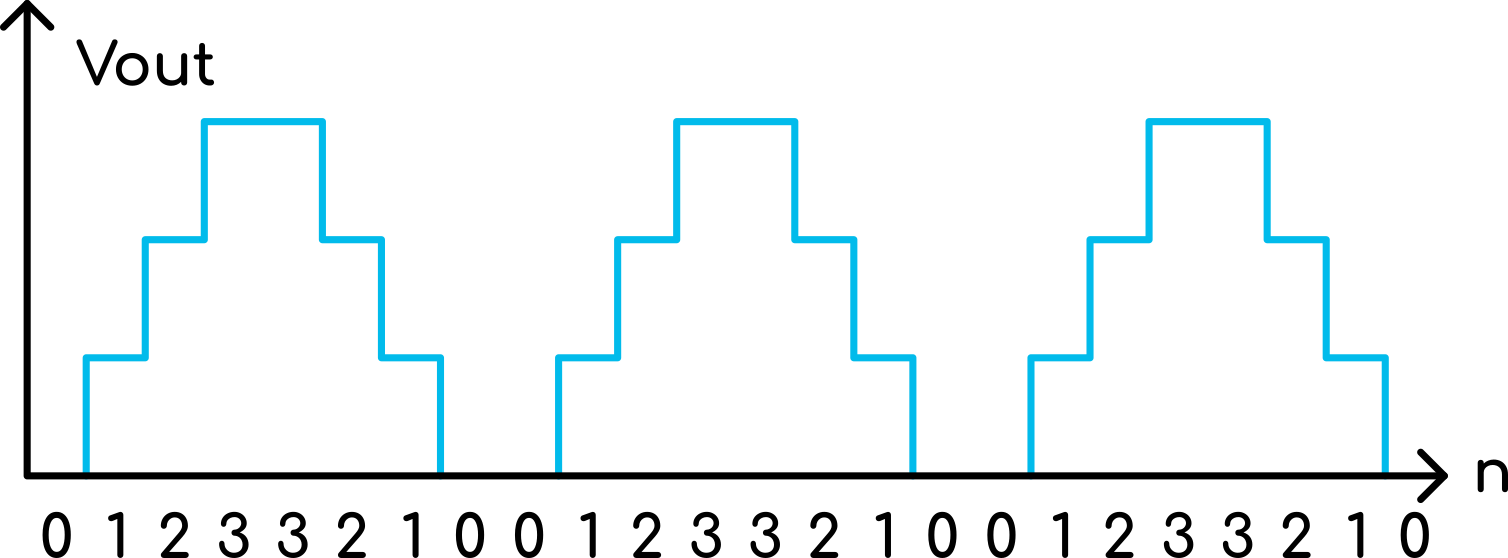
\includegraphics{graphs/low_res_triangle.png}
        \caption{Triangolo ottenuto con un contatore a 2 bit}
        \label{low_res_triangle}
    \end{subfigure}%
    \begin{subfigure}{.5\textwidth}
        \centering
        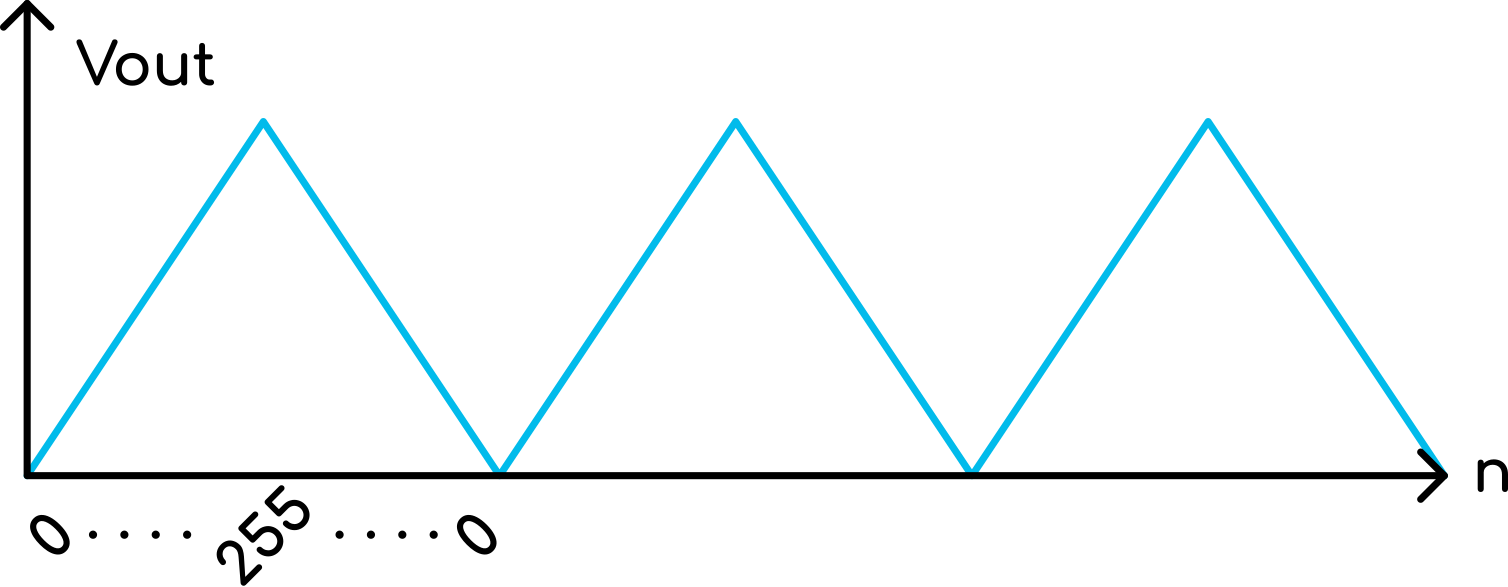
\includegraphics{graphs/high_res_triangle.png}
        \caption{Triangolo ottenuto con un contatore a 8 bit}
        \label{high_res_triangle}
    \end{subfigure}

    \caption{Confronto tra contatori bidirezionali con diverso numero di bit}
    \label{triangles}
\end{figure}

La configurazione del DAC rimane quella utilizzata per la rampa, rappresentata in figura
\ref{DAC_circuit}, va tuttavia fatta notare una importante differenza, ovvero che in questo
caso il numero di cicli di clock utilizzati è doppio rispetto a quello per la rampa. Infatti
dovranno essere eseguiti 256 conteggi verso l'alto e 256 conteggi verso il basso per effettuare
un singolo periodo di onda triangolare. Ne consegue quindi che anche la frequenza di clock
in ingresso a questo sottosistema dovrà essere doppia rispetto alla rampa, come risulta
evidente in figura \ref{steps}.
\medskip

\begin{figure}[ht]
    \centering

    \begin{subfigure}{.5\textwidth}
        \centering
        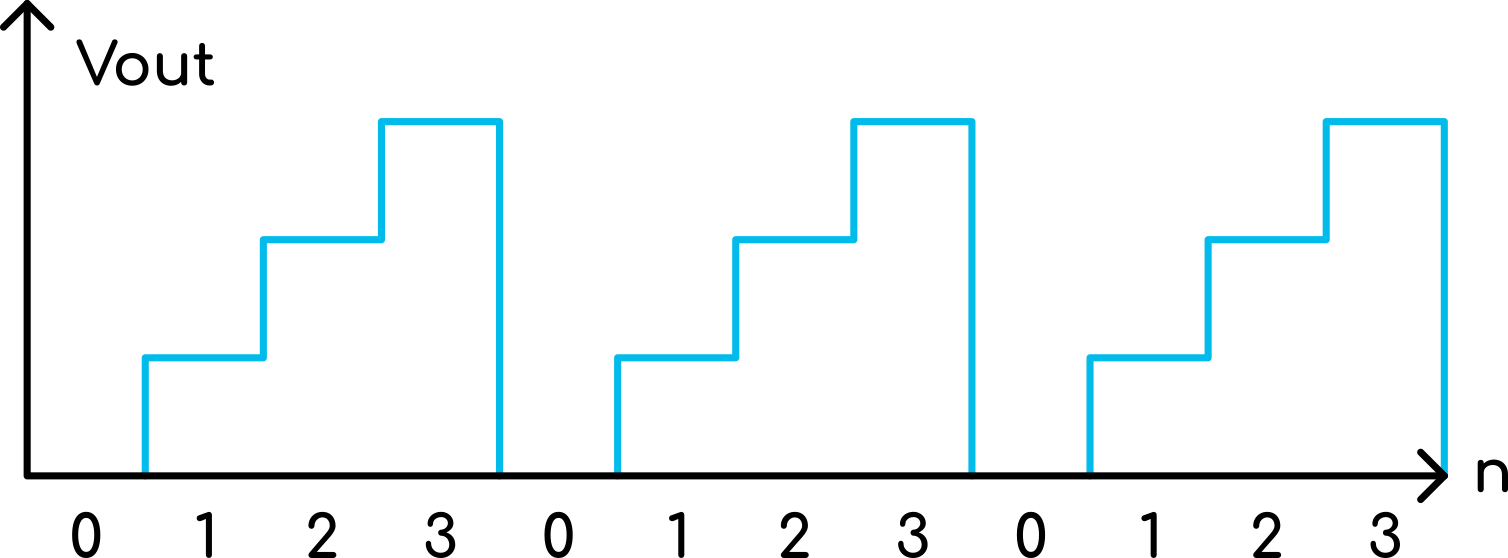
\includegraphics{graphs/low_res_ramp.png}
        \caption{Rampa ottenuta con un contatore a 2 bit}
    \end{subfigure}%
    \begin{subfigure}{.5\textwidth}
        \centering
        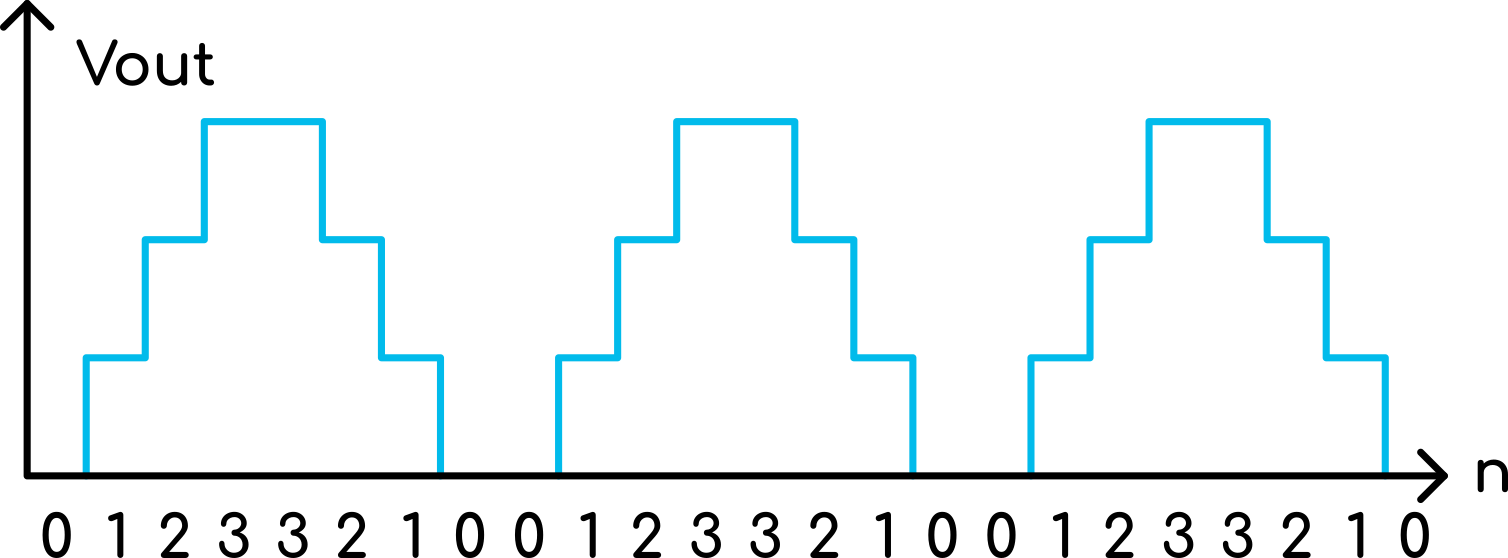
\includegraphics{graphs/low_res_triangle.png}
        \caption{Triangolo ottenuto con un contatore a 2 bit}
    \end{subfigure}

    \caption{Confronto del conteggio tra contatori unidirezionali e bidirezionali}
    \label{steps}
\end{figure}

%--------------------------------------------------------------------------------------------

\subsection*{Componenti Utilizzati e Schemi Elettrici}

L'unico componente diverso rispetto al circuito per la rampa è il contatore, che come già
detto deve essere bidirezionale. Si utilizzano due 74LS169 \cite{74ls169} in cascata con
la seguente configurazione:
\medskip

\begin{figure}[ht]
    \centering
    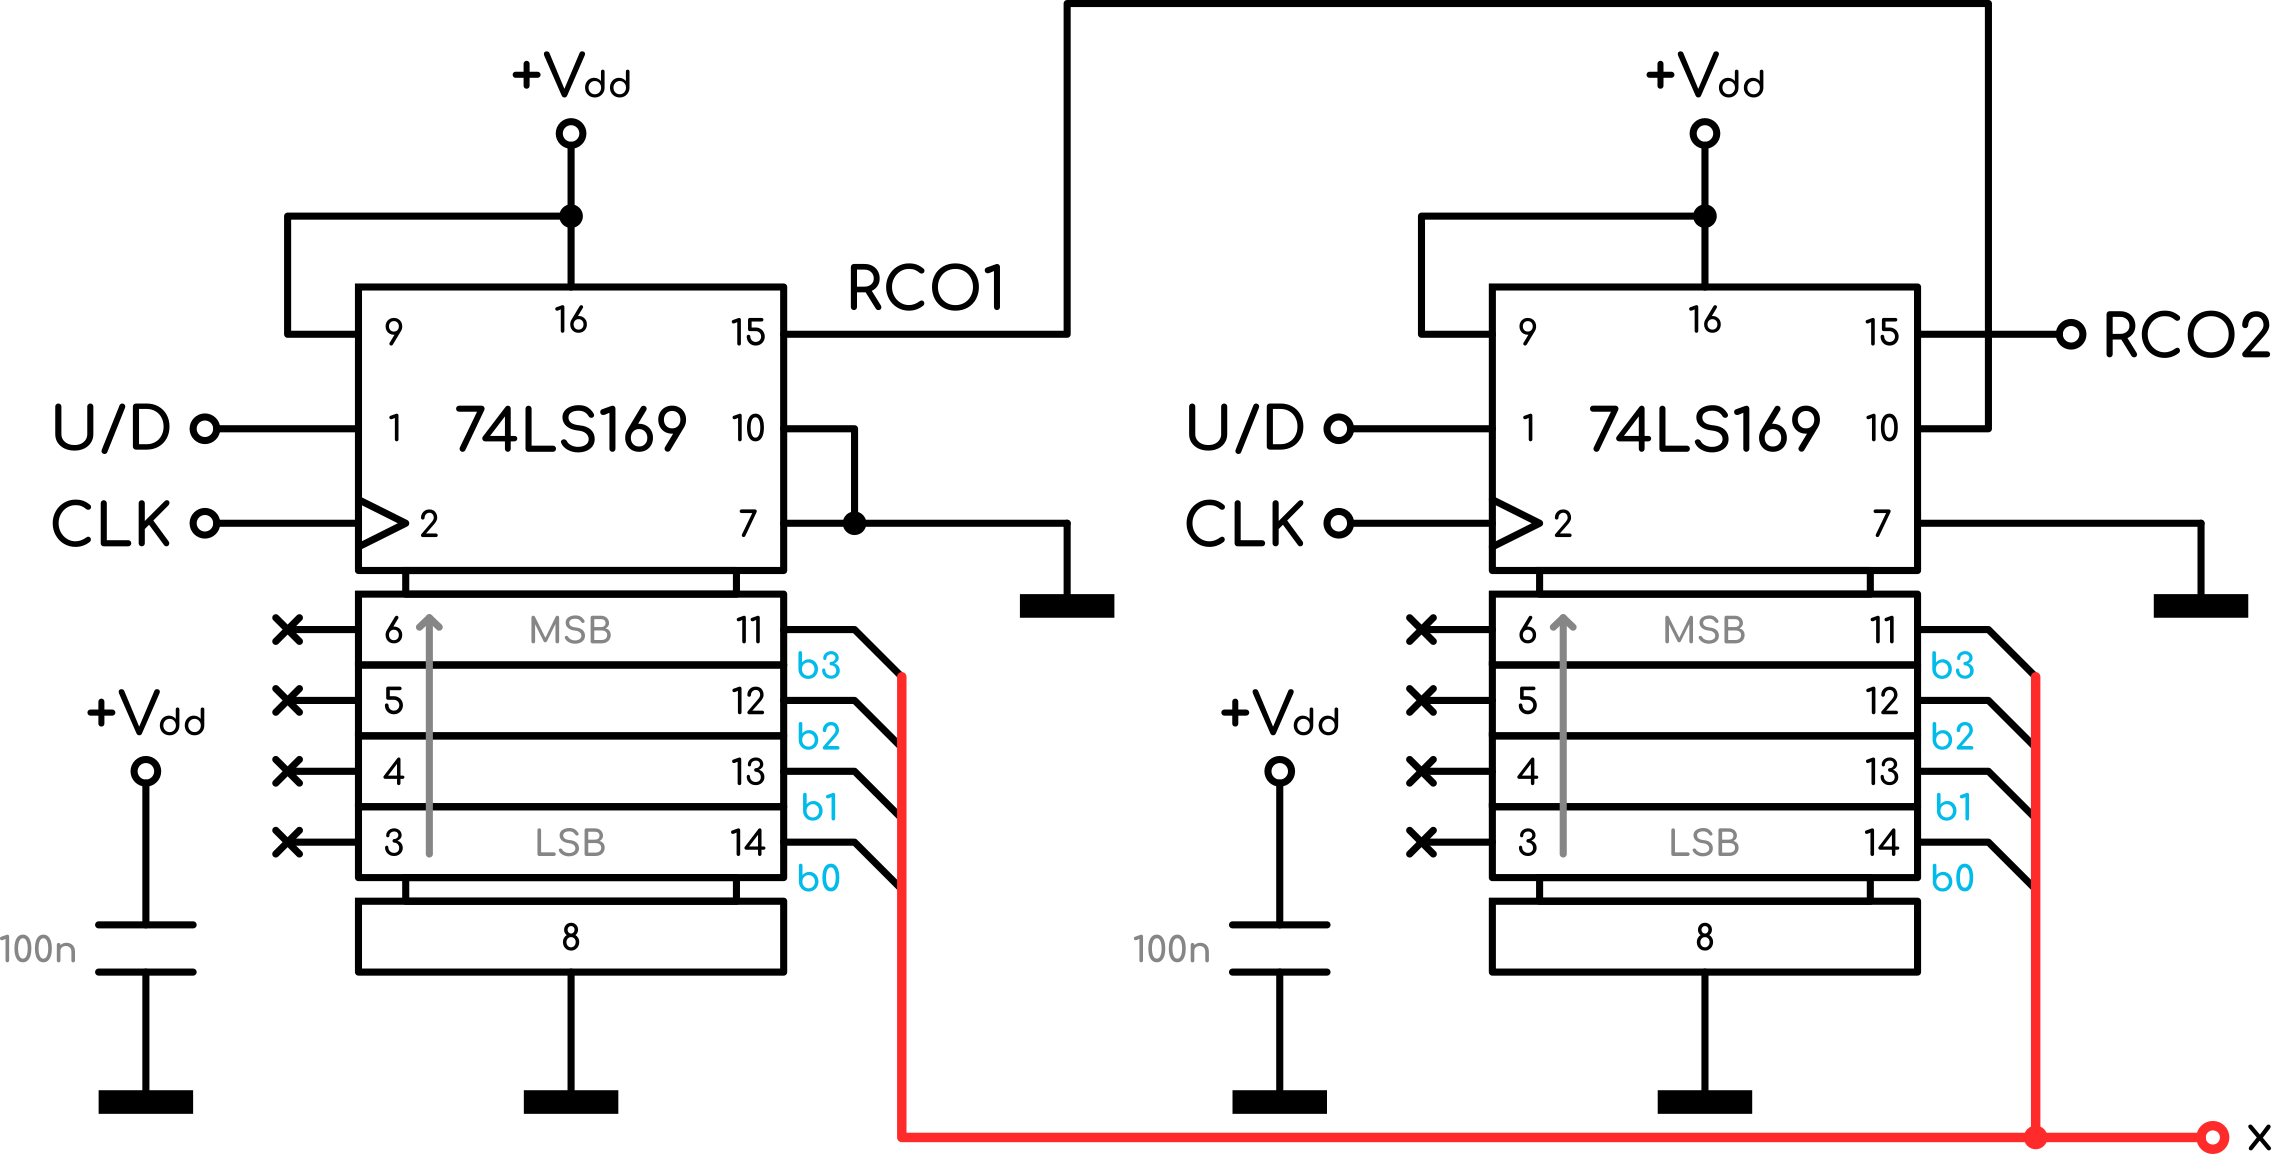
\includegraphics{circuits/triangle_counter_circuit.png}
    \caption{Schema elettrico dei contatori per l'onda triangolare, $V_{dd}=+5V$}
    \label{triangle_counter_circuit}
\end{figure}

Il componente utilizzato presenta anche degli ingressi per il preset del numero di partenza
(pin da 3 a 6), che però nel nostro caso non vengono utilizzati.

L'uscita denominata $RCO2$ verrà utilizzata per pilotare il verso del conteggio.

%--------------------------------------------------------------------------------------------

\subsection*{Risultati Pratici}

%--------------------------------------------------------------------------------------------

Andiamo ora a verificare la correttezza del circuito realizzato. Il setup di misura è il
seguente:
\medskip

% immagine setup misure rampa

Si osservano le seguenti forme d'onda:
\medskip

\begin{figure}[ht]
    \centering

    \begin{subfigure}{.5\textwidth}
        \centering
        
\includegraphics{misc/oscilloscope_placeholder.png}
        \caption{Acquisizione del segnale a triangolo reale}
        \label{acq_triangle}
    \end{subfigure}%
    \begin{subfigure}{.5\textwidth}
        \centering
        
\includegraphics{misc/oscilloscope_placeholder.png}
        \caption{Zoom degli step del triangolo acquisito e clock}
        \label{acq_triangle_steps}
    \end{subfigure}

    \caption{Acquisizioni del segnale a triangolo}
    \label{acq_triangle_signals}
\end{figure}

%--------------------------------------------------------------------------------------------

\section{Adattamento dei Segnali di Clock}

%--------------------------------------------------------------------------------------------

Si è visto come, per avere la stessa frequenza di segnale d'uscita, il contatore del
triangolo deve avere una frequenza di clock doppia rispetto a quella del contatore della
rampa. Questo problema si risolve facilmente utilizzando un divisore di frequenza,
ottenuto con un semplice toggle flip-flop (TFF).
\medskip

\begin{figure}[ht]
    \centering
    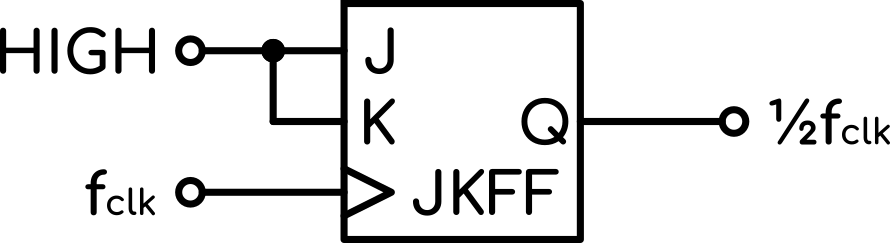
\includegraphics{block_diagrams/freq_divider_block_diagram.png}
    \caption{Schema a blocchi del divisore di frequenza}
    \label{freq_divider_block_diagram}
\end{figure}

Le specifiche sul segnale di clock ci impongono allora di generare un segnale a onda quadra
con frequenza variabile tra $\approx14kHz$ e $\approx3.6MHz$.

Invece, per fare in modo che il contatore del triangolo cambi effettivamente verso di conteggio
è necessario utilizzare un altro TFF collegato al segnale $RCO2$ invertito (poichè attivo a
livello logico basso) e all'ingresso $U/D$.
\medskip

\begin{figure}[ht]
    \centering
    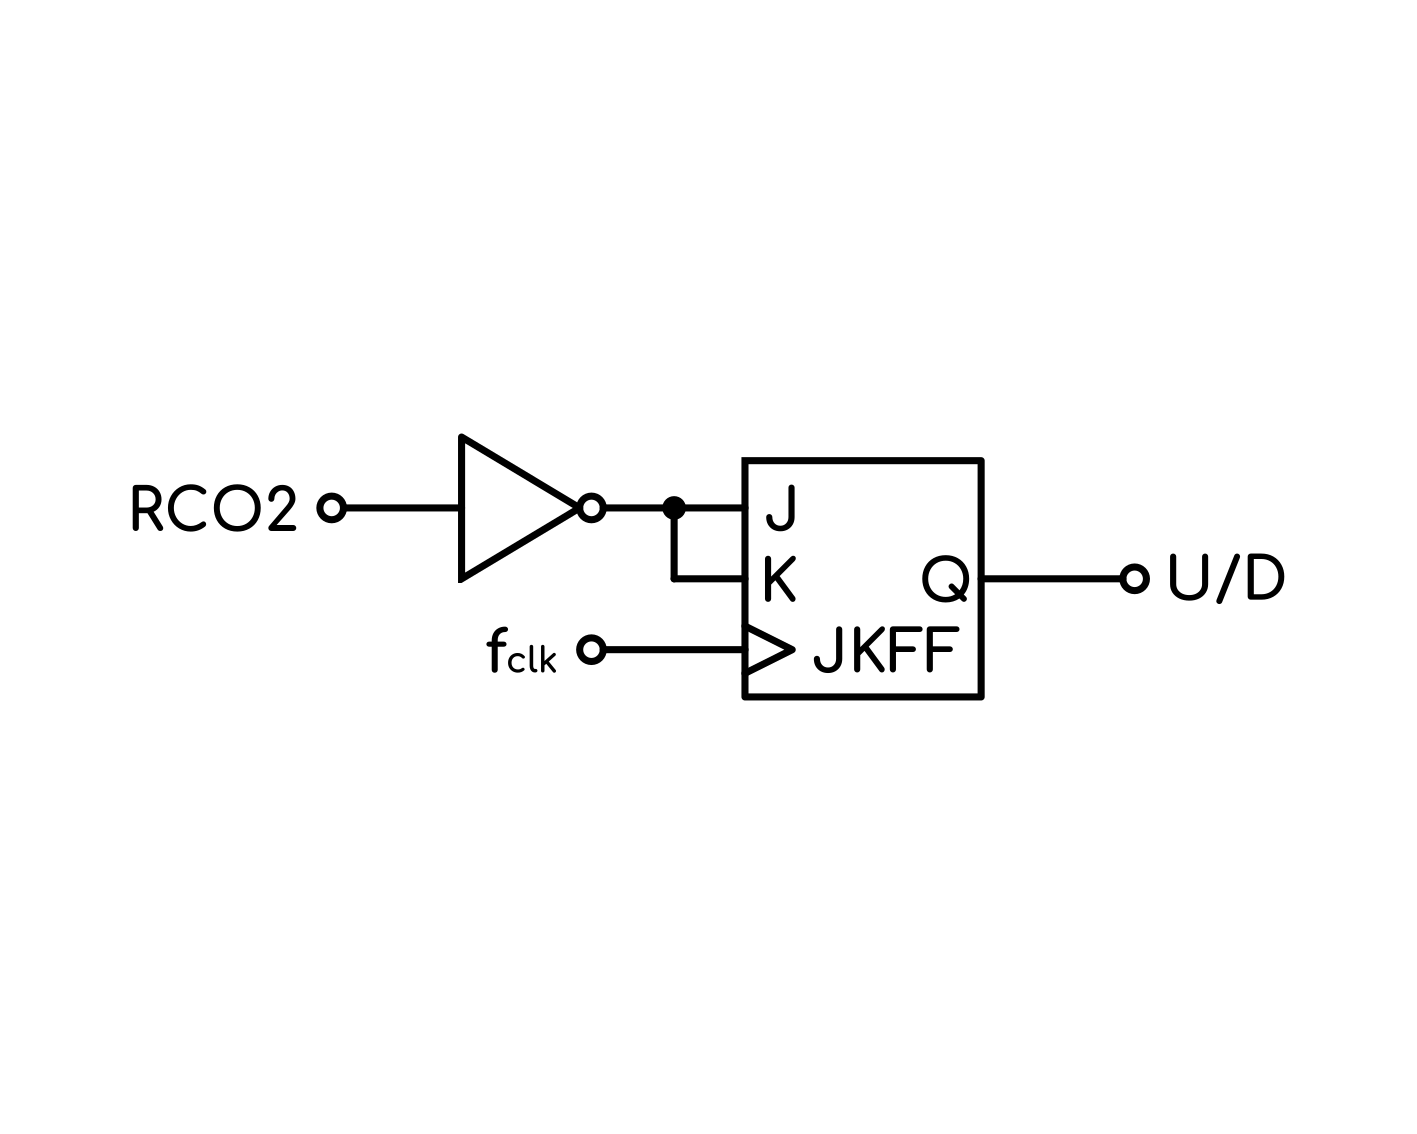
\includegraphics{block_diagrams/UD_block_diagram.png}
    \caption{Schema a blocchi del sistema per il segnale di pilotaggio}
    \label{UD_block_diagram}
\end{figure}

I componenti utilizzati per questo scopo sono:

\begin{itemize}
    \item Flip-Flop: 74HC73 \cite{74hc73};
    \item MOSFET: 2N7000 \cite{2n7000};
\end{itemize}

Il chip utilizzato per i flip-flop fornisce esattamente le 2 unità necessarie al nostro
scopo, mentre lo schema elettrico per l'inverter è rappresentato in figura
\ref{inverter_circuit}, dove il MOSFET utilizzato è compatibile con le tensioni logiche
presenti nel circuito.
\medskip

\begin{figure}[ht]
    \centering
    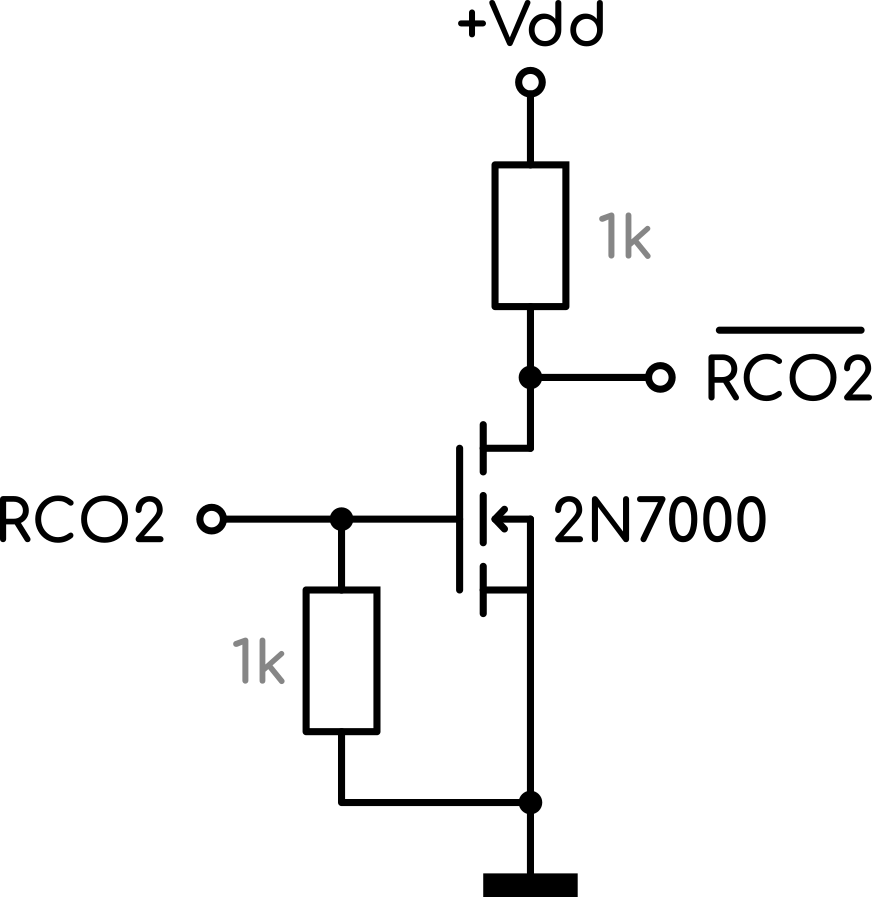
\includegraphics{circuits/inverter_circuit.png}
    \caption{Schema elettrico dell'inverter logico, $V_{dd}=+5V$}
    \label{inverter_circuit}
\end{figure}

A questo punto collegando tutti i pezzi discussi finora, otteniamo il nucleo fondamentale
del modulo, che ci permette di ottenere rampa e triangolo ad una frequenza proporzionale
a quella del clock in ingresso.
\medskip

\begin{figure}[ht]
    \centering
    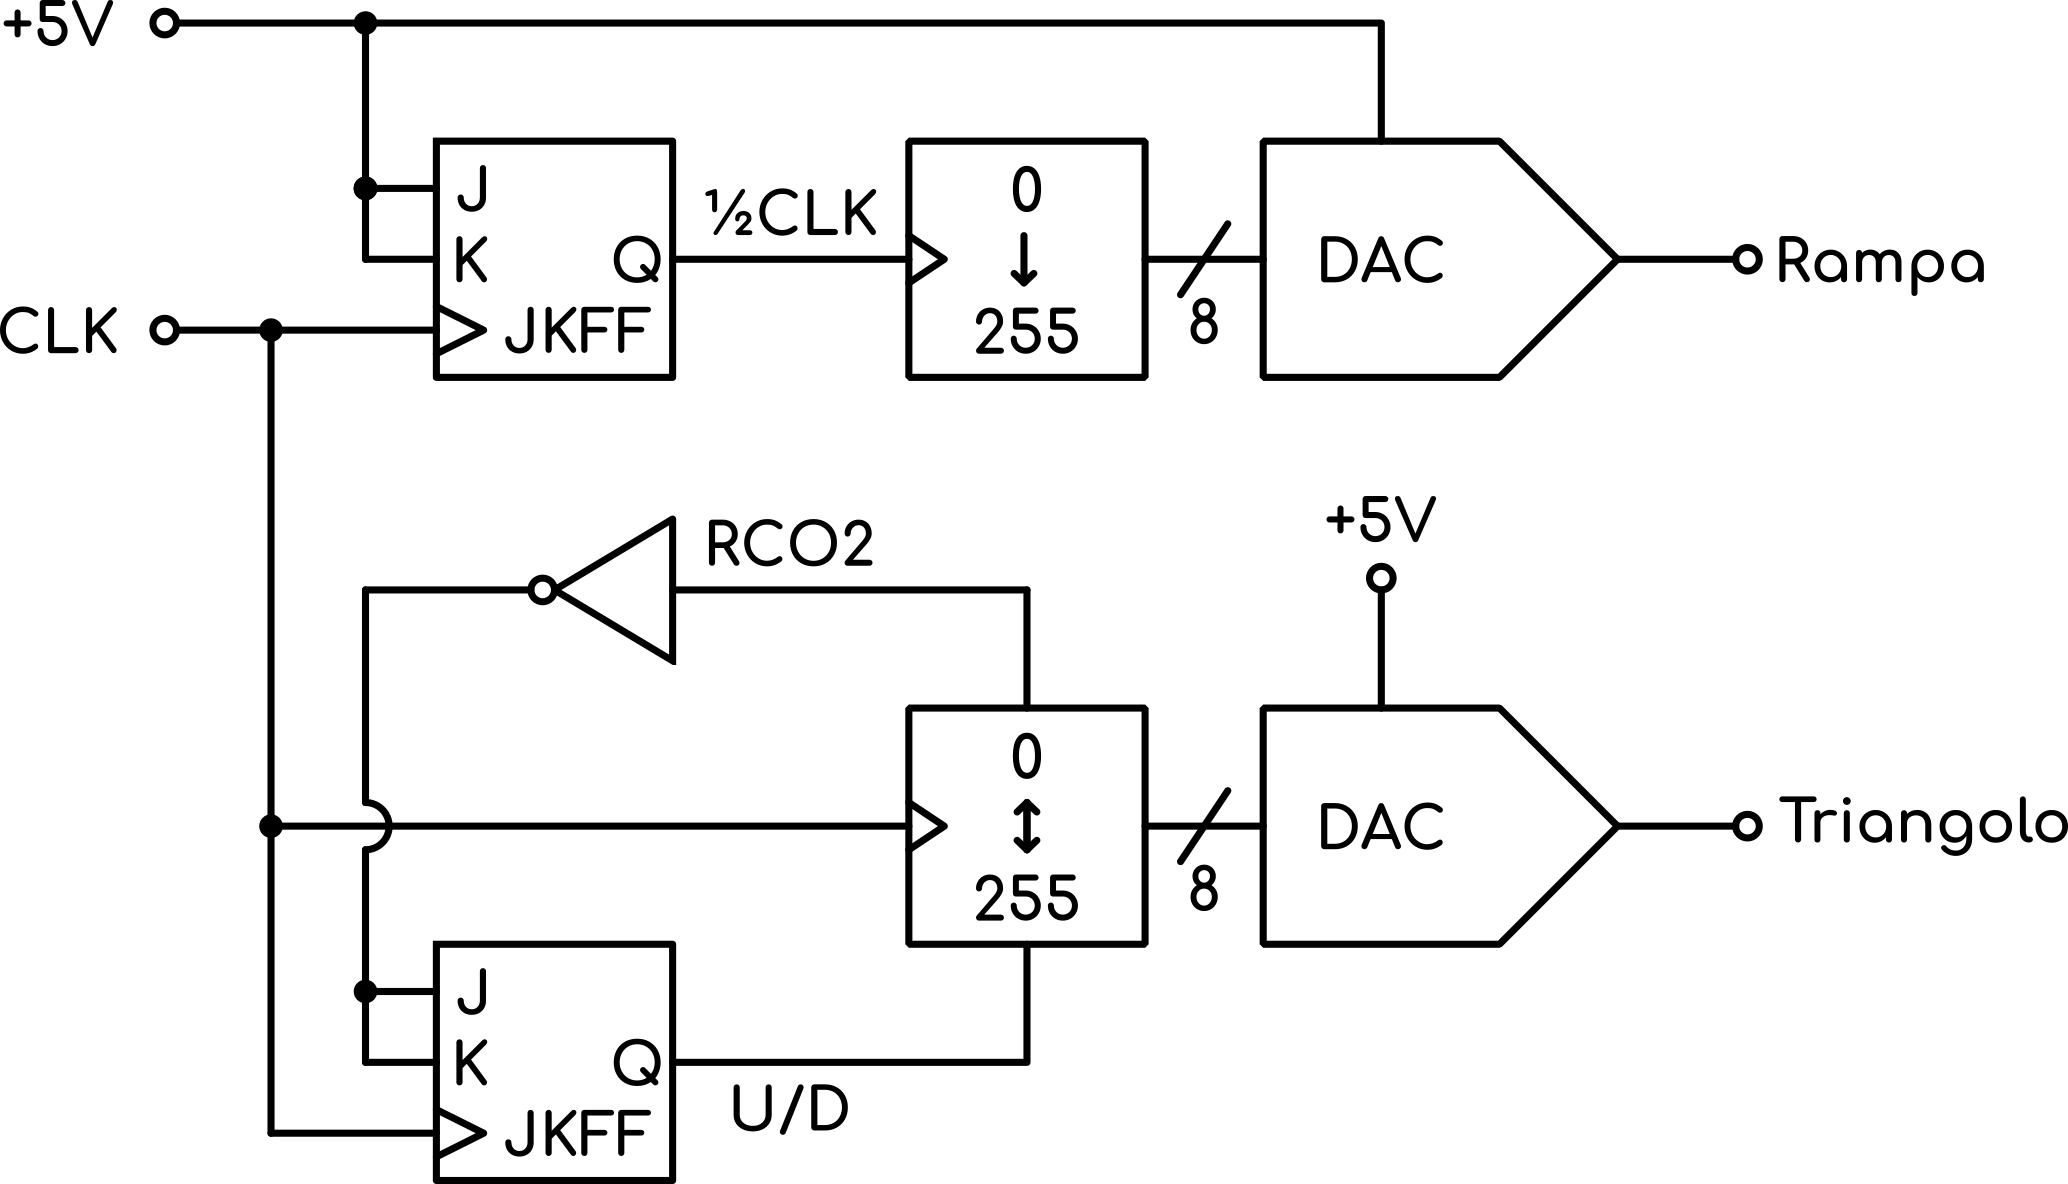
\includegraphics{block_diagrams/main_signals_block_diagam.png}
    \caption{Schema a blocchi del nucleo segnali}
    \label{main_signals_block_diagram}
\end{figure}

%--------------------------------------------------------------------------------------------
